\section{Evaluation}

\subsection{Detailed evaluation of examples}

In this section we discuss in full detail the execution trace
of the implementation of some examples. 

\subsubsection{Symbol elimination example}

Let us consider the following example from \cite{KAPUR2017} 
$\alpha_1 = \{f(z_1, v) = s_1, f(z_2, v) = s_2, f(f(y_1, v), f(y_2, v)) = t\}$
with the set of symbols to eliminate $U_1 = \{u\}$. The implementation produces the following
trace (slightly modified for presentation purposes) in order to compute 
the interpolant of $\alpha_1; U_1$:

\verbatiminput{../../Software/Cpp/EUFInterpolant/tests/traces/current_progress_example1.txt}

The interface offered by SMT solvers with interpolation features usually provide the 
conventional A-part, B-part format. In order to compare the results with the implementation two 
instances were tested so we can obtain interpolants from both systems:

\begin{itemize}
\item Problem instance: A-part : $\{f(z_1, v) = s_1, f(z_2, v) 
  = s_2, f(f(y_1, v), f(y_2, v)) = t\}$; B-part : 
  $\{z_1 = z_2, s_1 \neq s_2 \}$
\begin{itemize}
\item Z3: (or (= s2 s1) (not (= z2 z1)))
\item Mathsat: (not (and (= z1 z2) (not (= s1 s2))))
\item Our implemenation: ($\rightarrow$ (= z1 z2) (= s1 s2))
\end{itemize}

\item Problem instance: A-part : $\{f(z_1, v) = s_1, f(z_2, v) 
  = s_2, f(f(y_1, v), f(y_2, v)) = t\}$; 
  B-part : $\{z_1 = y_1, z_1 = y_2, f(s_1, s_1) \neq t\}$
\begin{itemize}
\item Z3: (or (= (f s1 s1) t) (not (= z1 y1)) (not (= y2 y1)))
\item Mathsat: (not (and (not (= t (f s1 s1))) (and (= z1 y1) (= z1 y2))))
\item Our implemenation: ($\rightarrow$ (and (= y1 y2) (= z1 y2) (= z1 y2)) (= t (f s1 s1))))
\end{itemize}

\end{itemize}

Clearly, the interpolant obtained by just eliminating the symbol $v$ implies
the outputs produced by Z3 and Mathsat for the previous problem instances.

\subsubsection{Simple example with disequality}

Let us consider another example from \cite{KAPUR2017} 
$\alpha_2 = \{f(x_1) \neq f(x_2)\}$
with the set of symbols to eliminate $U_2 = \{f\}$. The implementation produces the following
trace for $\alpha_2; U_2$:

\verbatiminput{../../Software/Cpp/EUFInterpolant/tests/traces/current_progress_example2.txt}

To compare our result with Z3 and Mathsat we 
included the B-part formula to be $\{x_1 = x_2\}$.
The interpolants obtained by these systems were the 
same, which was (not (= x1 x2)).

\subsection{Performance comparison with iZ3 and MathSat}\label{performance_euf}

This discuss will discuss a parametrized problem which will allows to test 
our implementation and constrast the execution with other interpolant generation
algorithms from Z3 and MathSat.

\begin{lemma} \label{performance_test_lemma}
  Let $x$ be a constant and $f$ an unary function in the EUF language. 
  For every $n \in \mathbb{N}$ the following conjunction is unsatisfiable:
  \begin{equation*}
    f^n(x) = f^{n+1}(x), f^2(x) = x, f(x) \neq x
  \end{equation*}
  where $f^n(x)$ denotes de application of the function $f$ n-times
  to the constant $x$.
\end{lemma}

\begin{proof}
  Applying the congruence and transitive rules to the equation $f^2(x) = x$, 
  we can prove that for any number $n$ the two following equations hold:
  $x = f^{2n}(x)$ and $f(x) = f^{2n+1}(x)$.

  At this point we distinguish two cases for $n$:

  \begin{itemize}
    \item Case $n$ is even: Then $\exists m \in \mathbb{N} . n = 2m$.
      So by choosing $n = m$ to the above sequence
      and by the axiom $f^{2m}(x) = f^{2m+1}(x)$ we have that
      $x = f(x)$.
    \item Case $n$ is odd: Similarly to the previous reasoning, 
      we can also infer the equation $f^{2m+1}(x) = f^{2m+2}(x)$
      by congruence, so $x = f(x)$.
    \end{itemize}

    In both cases the equation $x = f(x)$ reaches contradiction with the
    disequality $x \neq f(x)$.
\end{proof}

The interpolation pair for our performance test 
is $(f^n(x) = f^{n+1}(x) \land f^2(x) = x \land f(a) \neq a, x = a)$
for fixed $n \in \mathbb{N}$.
It is easy to see that the pair is inconsistent due to the lemma 
\ref{performance_test_lemma}. 

By lemma \ref{performance_test_lemma}
we can also see that the formula $x = a \rightarrow \bot$ is an 
interpolating formula for all fixed $n$ in this parametrized problem.
We designed this problem because it is easy to verify the 
correctness of output of the algorithms and to measure 
the time used by the algorithms for large values of $n$. 
We executed instances of this problem for values of $n$
in the range $\{1, \dots, 10000\}$ using a computer desktop
equipped with an Intel i7-9700 @ 4.70 GHz and 16Gb of memory. 
The output produced by the interpolant generation algorithms
were the expected formula.
The following graphs reports the time measured by the UNIX
utility $times$ of our implementation, iZ3, and the interpolation 
generation algorithm from Mathsat.

\begin{figure}
  \centering
  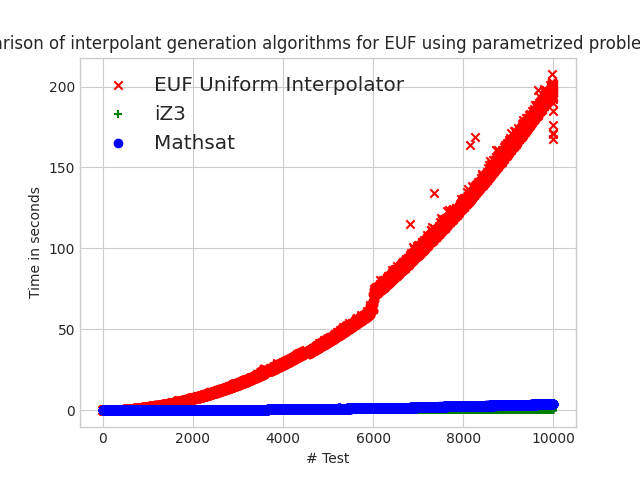
\includegraphics[scale=0.9]{figures/eufi_performance_graph}
  \caption{Performance comparison graph of EUF interpolant generation
  algorithms for paramatrized problem from section \ref{performance_euf}} 
  \label{performance_graph_euf}
\end{figure}

We noticed a quadractic behaviour in the graph for the time 
required by our implementation
and a linear behaviour by iZ3 and Mathsat. However, 
according to the following polynomial 
fitting computation, 
we noticed that for the case of our implementation, 
a linear fitting obtained a smaller 
quadratic error compared to the quadratic fitting;  
for the case of the Mathsat
results, a quadratic fitting obtained a smaller 
quadratic errror.

\begin{table}[h]
  \centering
  \begin{tabular}{ccc}
    \toprule
    {}                 & Error of linear fitting & Error of quadratic fitting \\
    \cmidrule{2-2} \cmidrule{3-3} \\
    iZ3                &  1.8723744548656934e-27 & 2.3456535579201815e-26     \\
    Mathsat            &  8.690566310635247e-23  & 7.576220133742597e-23      \\
    Our implementation &  2.5622746654442585e-20 & 6.648236698726508e-20      \\
    \bottomrule
  \end{tabular}
\end{table}

%%% Local Variables:
%%% mode: latex
%%% TeX-master: "main"
%%% End:
